\documentclass[journal]{IEEEtran}
\usepackage[pdftex]{graphicx}
\usepackage[cmex10]{amsmath}

% declare the path(s) where your graphic files are
\graphicspath{{./diagrams/}}

\begin{document}

% paper title
% can use linebreaks \\ within to get better formatting as desired
\title{Dynamic Load Balancing for\\Heterogeneous Systems}

% author names and IEEE memberships
\author{Kenneth~Lee,~Kyle~Morgan}%

% The paper headers
\markboth{CS 5504: Computer Architecture}{Final Project Paper, 5 December 2011}

% make the title area
\maketitle

\begin{abstract}
Leveraging maximimum performance from specialized hardware is one of the
major problems facing computer scientists today.  General-purpose computing
on graphics processing units (GPGPU) is a technique that is becoming
increasingly popular for handling computations typically performed by the
CPU.  However, many GPGPU algorithms place the entire workload on the GPU,
leaving the CPU idle for the duration of the computation.  This paper
investigates the effect various load-balancing schemes across the CPU and
GPU have on overall application performance.  Additionally, the discrete and
fused GPU architectures, and their impact on performance, will be investigated.
\end{abstract}

\section{Introduction}
% The very first letter is a 2 line initial drop letter followed
% by the rest of the first word in caps.
% 
% form to use if the first word consists of a single letter:
% \IEEEPARstart{A}{demo} file is ....
% 
% form to use if you need the single drop letter followed by
% normal text (unknown if ever used by IEEE):
% \IEEEPARstart{A}{}demo file is ....
% 
% Some journals put the first two words in caps:
% \IEEEPARstart{T}{his demo} file is ....
\IEEEPARstart{L}{everaging} the maximum performance from specialized hardware is one
of the major challenges computer scientists face today.  The unique hardware architecture
of the Graphics Processing Unit (GPU) gives it a place as a massively parallel hardware
accelerator.  However, because of the difficulty in programming for this hardware,
most of the effort is spent on trying to achieve performance from the GPU, while
leaving the CPU unused.  By also using the CPU to process a smaller part of the
data we can achieve higher utilization of resources and therefore increase program
performance.

GPU+CPU co-processing hardly a new idea.  Jimenez et al. \cite{jimenez} present a
dynamic library which can be used in a system to dynamically schedule tasks for GPU
computation across various processes. The method describes only looks at optimizing
usage of the GPU across the whole system, instead of optimizing a single application’s
performance. The StarPU system, on the other hand, presents a method of co-processing
and load balancing on a per application basis \cite{augonnet}. They show that by using an
appropriate model for the load balancing, they are able to achieve improvements in
speed for applications which call for code acceleration multiple times.  We intend
to extend this work to improve the speed of each kernel execution by splitting the
work of that kernel over the capable resources, similar to the schemes used by OpenMP.
Both of these papers address data transfer times as a major cost of GPU computing.
Using the new AMD Fusion architecture, which fuses the CPU and GPU onto a single die,
we may be able to eliminate or greatly reduce this cost, which will impact the overhead
of GPU+CPU co-processing.

We expect that by using GPU+CPU processing we will improve the performance of the
application, when compared to CPU-only or GPU-only.  We will measure performance of the
application using a wall time clock.  We also hypothesize that the fused GPU+CPU
architecture will allow for lower overhead for load balancing.

\section{Motivation}
Lorem ipsum dolor sit amet, consectetur adipisicing elit, sed do
eiusmod tempor incididunt ut labore et dolore magna aliqua. Ut
enim ad minim veniam, quis nostrud exercitation ullamco laboris
nisi ut aliquip ex ea commodo consequat. Duis aute irure dolor
in reprehenderit in voluptate velit esse cillum dolore eu fugiat
nulla pariatur. Excepteur sint occaecat cupidatat non proident,
sunt in culpa qui officia deserunt mollit anim id est laborum.

\section{Architecture Overview}
In this section we discuss the different architectures of the experimental
machines under test.  We will discuss CPU, GPU, and APU architectures in
terms of major differences that affect the performance of the device.  

\subsection{CPU Architecture}
The CPU architecture is designed as a low latency architecture.  To facilitate
the needs for low latency application performance, a series of hierarchical 
caches have been designed to hide memory access costs, the most common cause
of latency in single-threaded applications on modern architectures.  Each core
of the CPU typically only runs one or two hardware-enabled threads to reduce
cache pollution, thus avoiding latency.  An example CPU architecture is given
by Figure \ref{fig:cpu_arch}.

The use of the Single Instruction Multiple Data (SIMD) paradigm enables increased
performance on these devices by increasing data throughput for data parallel
applications.

\subsection{GPU Architecture}
The GPU almost acts a foil to the CPU architecture.  Instead of optimizing the
architecture of the device to increase performance of a single thread, the GPU
architecture is specifically designed for large throughput performance.  

The memory hierarchy for the GPU architecture is given by Figure \ref{fig:gpu_arch}.

\begin{figure}[!t]
\centering
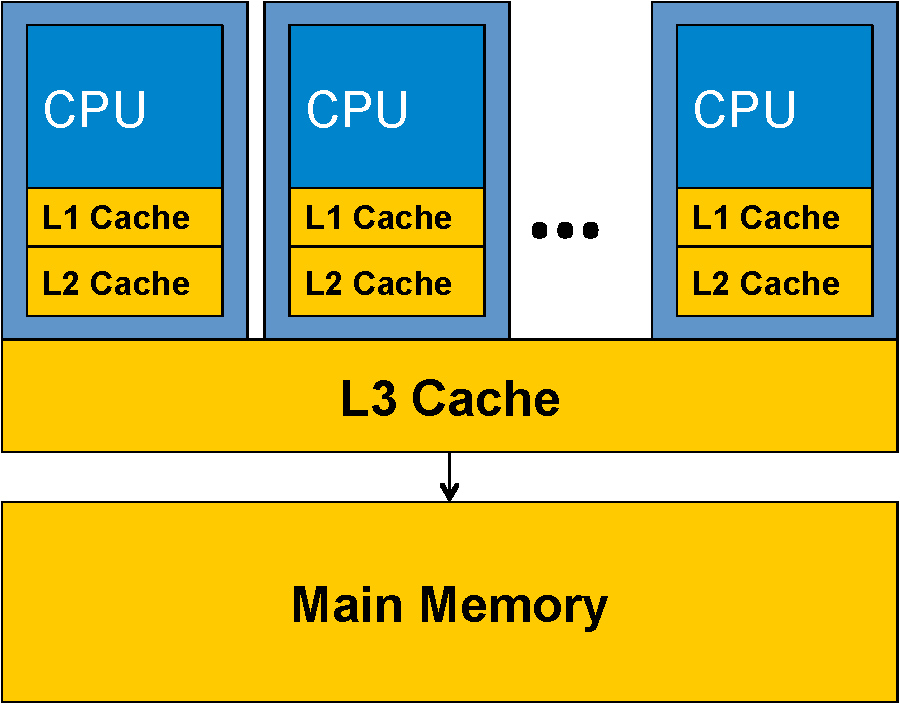
\includegraphics[width=2.5in]{cpu_architecture}
\caption{CPU Architecture}
\label{fig:cpu_arch}
\end{figure}

\begin{figure}[!t]
\centering
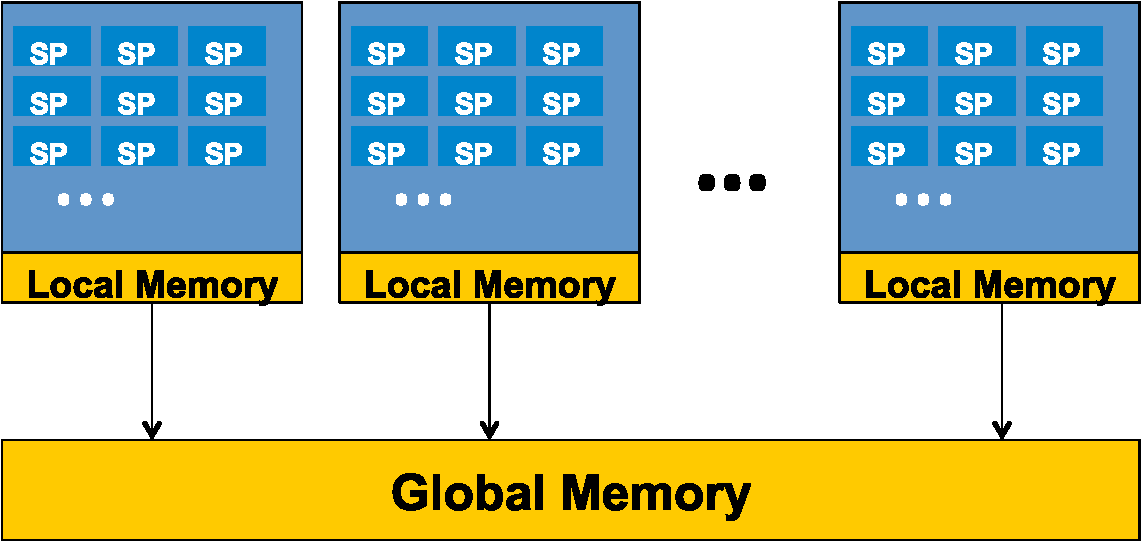
\includegraphics[width=2.5in]{gpu_architecture}
\caption{GPU Architecture}
\label{fig:gpu_arch}
\end{figure}

\subsection{APU Architecture}
Lorem ipsum dolor sit amet, consectetur adipisicing elit, sed do
eiusmod tempor incididunt ut labore et dolore magna aliqua. Ut
enim ad minim veniam, quis nostrud exercitation ullamco laboris
nisi ut aliquip ex ea commodo consequat. Duis aute irure dolor
in reprehenderit in voluptate velit esse cillum dolore eu fugiat
nulla pariatur. Excepteur sint occaecat cupidatat non proident,
sunt in culpa qui officia deserunt mollit anim id est laborum.

\section{Related Work}
Ryoo et al. discuss optimization strategies for GPU versus CPU runtime
systems~\cite{Ryoo2007}.  However, their research is based on a GPU-only
or CPU-only implementation instead of a heterogeneous approach.  The work
presented in ~\cite{Jablin2011} describes a runtime and compiled framework
for improving memory access latency and reducing data transfer overhead
for GPU kernels.  Our work differs from this, because the kernel execution
was still being performed soley on the GPU, whereas our work investigates
kernel execution on multiple devices.

Computation via heterogeneous systems is a relatively new research area for
high performance computing.  The various frameworks and large number of
different accelerator devices can make this quite difficult for application
programmers to manage.  The StarPU system~\cite{Augonnet2009} presents a 
framework to allow for programmers to write numerical codelets and have them
automatically run on a heterogeneous system.  Scheduling work for this system
is one of the most difficult parts of the system, because of the various
overheads for work-sharing schemes. We simplify this work, by looking at a
two-device system, and focus on the performance characteristics of different
scheduling scheme.  Verner et al. use this approach to create a high-throughput
low-lantecy heterogeneous encryption system~\cite{Verner2011}. 

Jimenez et al.~\cite{Jimenez2009} present a dynamic library which can be used
in a system to dynamically schedule tasks for GPU computation across various
processes. The method describes only looks at optimizing usage of the GPU across
the whole system, instead of optimizing a single application's performance.

% An example of a floating figure using the graphicx package.
% Note that \label must occur AFTER (or within) \caption.
% For figures, \caption should occur after the \includegraphics.
% Note that IEEEtran v1.7 and later has special internal code that
% is designed to preserve the operation of \label within \caption
% even when the captionsoff option is in effect. However, because
% of issues like this, it may be the safest practice to put all your
% \label just after \caption rather than within \caption{}.
%
% Reminder: the "draftcls" or "draftclsnofoot", not "draft", class
% option should be used if it is desired that the figures are to be
% displayed while in draft mode.
%
%\begin{figure}[!t]
%\centering
%\includegraphics[width=2.5in]{myfigure}
% where an .eps filename suffix will be assumed under latex, 
% and a .pdf suffix will be assumed for pdflatex; or what has been declared
% via \DeclareGraphicsExtensions.
%\caption{Simulation Results}
%\label{fig_sim}
%\end{figure}

% Note that IEEE typically puts floats only at the top, even when this
% results in a large percentage of a column being occupied by floats.


% An example of a double column floating figure using two subfigures.
% (The subfig.sty package must be loaded for this to work.)
% The subfigure \label commands are set within each subfloat command, the
% \label for the overall figure must come after \caption.
% \hfil must be used as a separator to get equal spacing.
% The subfigure.sty package works much the same way, except \subfigure is
% used instead of \subfloat.
%
%\begin{figure*}[!t]
%\centerline{\subfloat[Case I]\includegraphics[width=2.5in]{subfigcase1}%
%\label{fig_first_case}}
%\hfil
%\subfloat[Case II]{\includegraphics[width=2.5in]{subfigcase2}%
%\label{fig_second_case}}}
%\caption{Simulation results}
%\label{fig_sim}
%\end{figure*}
%
% Note that often IEEE papers with subfigures do not employ subfigure
% captions (using the optional argument to \subfloat), but instead will
% reference/describe all of them (a), (b), etc., within the main caption.


% An example of a floating table. Note that, for IEEE style tables, the 
% \caption command should come BEFORE the table. Table text will default to
% \footnotesize as IEEE normally uses this smaller font for tables.
% The \label must come after \caption as always.
%
%\begin{table}[!t]
%% increase table row spacing, adjust to taste
%\renewcommand{\arraystretch}{1.3}
% if using array.sty, it might be a good idea to tweak the value of
% \extrarowheight as needed to properly center the text within the cells
%\caption{An Example of a Table}
%\label{table_example}
%\centering
%% Some packages, such as MDW tools, offer better commands for making tables
%% than the plain LaTeX2e tabular which is used here.
%\begin{tabular}{|c||c|}
%\hline
%One & Two\\
%\hline
%Three & Four\\
%\hline
%\end{tabular}
%\end{table}


% Note that IEEE does not put floats in the very first column - or typically
% anywhere on the first page for that matter. Also, in-text middle ("here")
% positioning is not used. Most IEEE journals use top floats exclusively.
% Note that, LaTeX2e, unlike IEEE journals, places footnotes above bottom
% floats. This can be corrected via the \fnbelowfloat command of the
% stfloats package.



\section{Conclusion}
Lorem ipsum dolor sit amet, consectetur adipisicing elit, sed do
eiusmod tempor incididunt ut labore et dolore magna aliqua. Ut
enim ad minim veniam, quis nostrud exercitation ullamco laboris
nisi ut aliquip ex ea commodo consequat. Duis aute irure dolor
in reprehenderit in voluptate velit esse cillum dolore eu fugiat
nulla pariatur. Excepteur sint occaecat cupidatat non proident,
sunt in culpa qui officia deserunt mollit anim id est laborum.

\begin{thebibliography}{1}

\bibitem{augonnet}
C.~Augonnet, S.~Thibault, R.~Namyst, and P.A.~Wacrenier,
``StarPU: A Unified Platform for Task Scheduling on Heterogeneous Multicore Architectures'' in
\emph{Proceedings of the 15th International Euro-Par Conference on Parallel Processing}, 2009, pp. 863-874.

\bibitem{che}
S.~Che, M.~Boyer, J.~Meng, D.~Tarjan, J.W.~Sheaffer, S.H.~Lee, and K.~Skadron,
``Rodinia: A benchmark suite for heterogeneous computing'' in
\emph{Proceedings of the 2009 IEEE International Symposium on Workload Characterization (IISWC)}, 2009, pp. 44-54.

\bibitem{danalis}
A.~Danalis, G.~Marin, C.~McCurdy, J.S.~Meredith, P.C.~Roth, K.~Spafford, V.~Tipparaju, and J.S.~Vetter,
``The Scalable Heterogeneous Computing (SHOC) benchmark suite'' in
\emph{Proceedings of the 3rd Workshop on General-Purpose Computation on Graphics Processing Units}, 2010, pp. 63-74.

\bibitem{jimenez}
V.J.~Jiménez, L.~Villanova, I.~Gelado, M.~Gil, G.~Fursin, and N.~Navarro,
``Predictive Runtime Code Scheduling for Heterogeneous Architectures,'' in
\emph{Proceedings of the 4th International Conference on High Performance Embedded
Architectures and Compilers}, 2009, pp. 19-33.

\end{thebibliography}

\newpage
\appendix[Team Member Contributions]
Kenneth Lee did A, B, C.  Kyle Morgan did X, Y, Z.
\end{document}
